\documentclass[14pt, a4paper, titlepage, fleqn]{extarticle}

\usepackage{style}
\usepackage{titlepage}

\everymath{\displaystyle}

\title{Контрольная работа по численному дифференцированию asd }
\author{Держапольский Юрий Витальевич \\ Группа Б9121-01.03.02сп}
\date{}

\begin{document}

    \fefutitlepage{ОТЧЁТ}{к лабораторной работе №3 по дисциплине\\«Дифференциальные уравнения»}
    {01.03.02 <<Прикладная математика и информатика>>}{Б9121-01.03.02сп(1)}{Держапольский Ю.В.}

    \tableofcontents

    \pagebreak

    \section{Введение}
        В этой лабораторной работе мы будем решать дифференциальные 
        уравнения, неразрешённые относительно производной, находить значение
        функции и строить её график с помощью производной, 
        а также решать дифференциальные уравнения высших
        порядков, верстая решения в \LaTeX.

    \pagebreak

    \section{Задание 1}
        \subsection{Постановка задачи}
            Для следующих дифференциальных уравнений указать вид,
            дать характеристику и найти общее решение с помощью программ
            компьютерной математики:

            \begin{enumerate}
                \item \( (r-r') \ln{r} = r' \left( \varphi - \ln{r'} \right); \)
                \item \( \tan{\frac{r}{r'}} = \ln{r}; \)
                \item \( r = \frac{3}{2} \varphi r' + e^{r'}; \)
                \item \( \dot{x}^2 - 2x \dot{x} = x^2 \cdot \left( e^{2t} - 1 \right); \)
                \item \( \ln{\theta} = \ln{r'} + r'^2 - 1; \)
            \end{enumerate}

        
        \subsection{Решение}
            \begin{enumerate}
                \item \( (r-r') \ln{r} = r' \left( \varphi - \ln{r'} \right); \)
                
                    \textit{Вид уравнения:} \( F \left( \varphi, r, r' \right) = 0; \)

                    \textit{Характеристика уравнения:}
                        Полное неразрешенное относительно производной;

                    \textit{Общее решение:} \( r^C = C e^\varphi. \)

                \item \( \tan{\frac{r}{r'}} = \ln{r}; \)
                
                    \textit{Вид уравнения:} \( F \left(r, r' \right) = 0; \)

                    \textit{Характеристика уравнения:}
                        Неразрешенное относительно производной, не содержащее аргумента;

                    \textit{Общее решение:} \( r e^{\arctg{\left( \ln r \right)}} = C e^\varphi \sqrt{\ln^2{r} + 1}. \)
                

                \item \( r = \frac{3}{2} \varphi r' + e^{r'}; \)
                
                    \textit{Вид уравнения:} \( F \left( \varphi, r, r' \right) = 0; \)

                    \textit{Характеристика уравнения:}
                        Уравнение Лагранжа;

                    \textit{Общее решение:} 
                        \(
                            \left\lbrace
                                \begin{aligned}
                                    r &= \frac{3C - \left(4p^2 - 12p + 12\right) e^p}{2p^2}, \\
                                    \varphi &= \frac{C - \left( 2p^2 - 4p + 4 \right)e^p}{p^3}.
                                \end{aligned}
                            \right.    
                        \)

                \item \( \dot{x}^2 - 2x \dot{x} = x^2 \cdot \left( e^{2t} - 1 \right); \)
                
                    \textit{Вид уравнения:} \( F \left( t, x, \dot{x} \right) = 0; \)

                    \textit{Характеристика уравнения:}
                        Полное неразрешенное относительно производной;

                    \textit{Общее решение:} \( \ln{x} = t \pm e^t + C. \)

                
                \item \( \ln{\theta} = \ln{r'} + r'^2 - 1; \)
                
                    \textit{Вид уравнения:} \( F \left( \theta, r' \right) = 0; \)

                    \textit{Характеристика уравнения:}
                        Неразрешенное относительно производной, не содержащее функции;

                    \textit{Общее решение:}
                        \(
                            \left\lbrace
                                \begin{aligned}
                                    \theta &= p e^{p^2-1}, \\
                                    r &= \left( p^2 - \frac{1}{2} \right) e^{p^2-1} + C.
                                \end{aligned}
                            \right.    
                        \)

            \end{enumerate}

            
    \pagebreak

    \section{Задание 2}
        \subsection{Постановка задачи}
            Разрешить следующие уравнения относительно производной и, 
            используя метод Эйлера, найти значение функции в точке. 
            Нарисовать график искомой функции. 
            Реализацию решения проводить на языке <<C++>>:

            \begin{enumerate}
                \item \( \sec^2{(1 -y- x)} = y'^2 - \tan{xy} + 2; \quad y \left( \frac{\pi}{4} \right) = 1, ~ y \left( \frac{\pi}{3} \right) = ?;  \)
                \item \( e^{x-y} = \cos\big( y' \sin{x} - \tan^2(\sec{xy}) - \tan{y} \big); \quad y \left( \frac{\pi}{3} \right) = \ln 7, ~ y(1) = ?. \)
            \end{enumerate}

        
        \subsection{Решение}
            \begin{enumerate}
                \item \( \sec^2{(1 -y- x)} = y'^2 - \tan{xy} + 2; \quad y \left( \frac{\pi}{4} \right) = 1, ~ y \left( \frac{\pi}{3} \right) = ?;  \)
                    \label{eq1}

                    \textit{Разрешённое уравнение:}
                        \( y' = \pm \sqrt{\sec^2 \left( 1 - y - x \right) + \tan{xy} - 2}; \)

                    \textit{Значение функции:}
                        \( \left[
                            \begin{aligned}
                                &1.85955\dots, \\
                                &0.737429\dots
                            \end{aligned}
                        \right. \)

                    \begin{figure}[H]
                        \centering
                        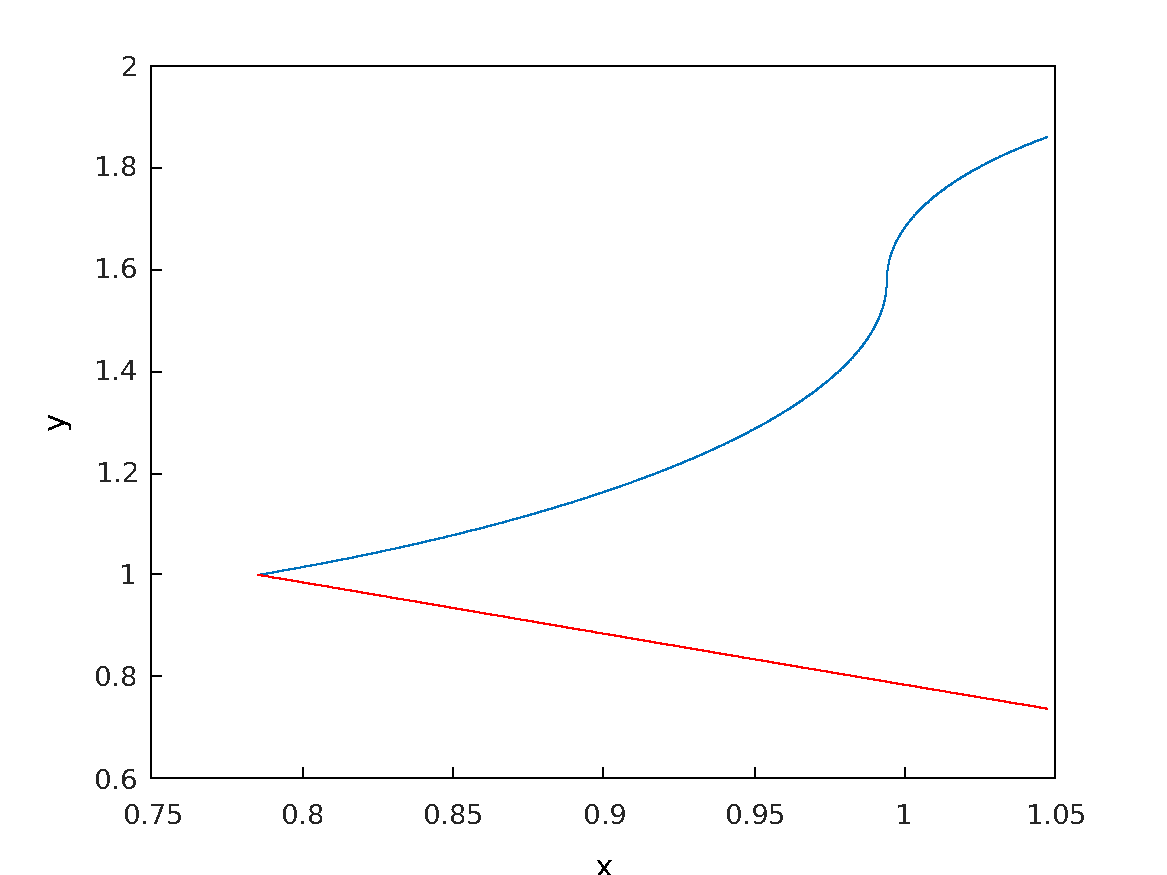
\includegraphics[width=10cm]{pictures/graph2_1.pdf}
                        \caption{График решений уравнения (\ref{eq1})}
                    \end{figure}

                    \pagebreak
                    \lstinputlisting[language=C++,
                        caption=Код программы,
                        style=Cpps,
                        basicstyle=\footnotesize\ttfamily,
                        frame=lines]{code/2_1.cpp}

                \pagebreak
                

                \item \( e^{x-y} = \cos\big( y' \sin{x} - \tan^2(\sec{xy}) - \tan{y} \big); \quad y \left( \frac{\pi}{3} \right) = \ln 7, ~ y(1) = ?; \)
                    \label{eq2}

                    \textit{Разрешённое уравнение:}
                        \( y' = \frac{\arccos \left( e^{x-y} \right) + \tan^2 ( \sec{xy} ) + \tan y}{\sin x}; \)

                    \textit{Значение функции:}
                        \( 1.97059\dots \)

                    \begin{figure}[H]
                        \centering
                        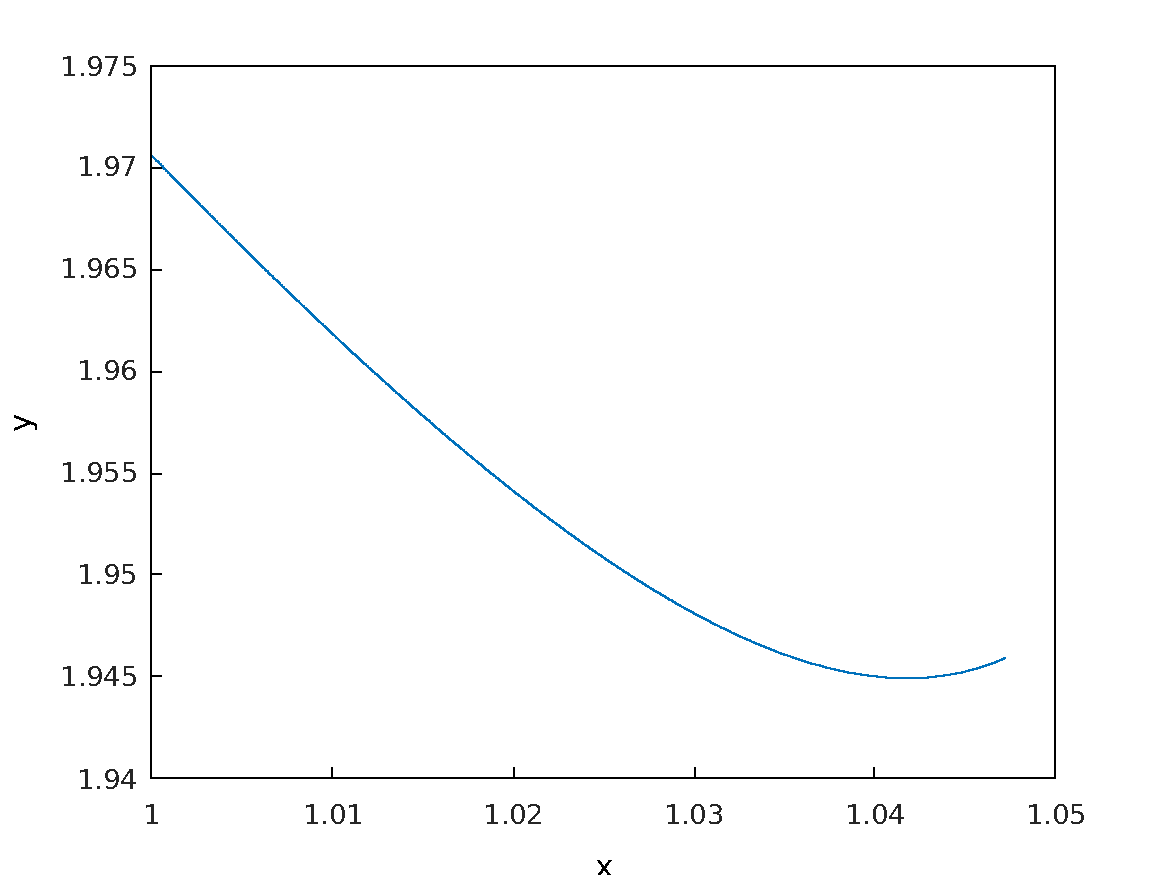
\includegraphics[width=10cm]{pictures/graph2_2.pdf}
                        \caption{График решений уравнения (\ref{eq2})}
                    \end{figure}

                    \pagebreak
                    \lstinputlisting[language=C++,
                        caption=Код программы,
                        style=Cpps,
                        basicstyle=\footnotesize\ttfamily,
                        frame=lines]{code/2_2.cpp}

            \end{enumerate}



    \pagebreak

    \section{Задание 3}
        \subsection{Постановка задачи}
            Для следующих дифференциальных уравнений определить тип, 
            дать характеристику и найти общее решение с помощью программ 
            компьютерной математики:

            \begin{enumerate}
                \item \( y'' \cdot \cos{y} = y'^2 \cdot \cot{y}; \)
                \item \( u^2 + 4tu \dot{u} + t^2 \dot{u}^2 + t^2 u \ddot{u} = 2tu \left( u + t \dot{u} \right) \cdot \tan{t}; ~ [z = \tan{t}]; \)
                \item \( \frac{\ddot{x}}{\dot{x}^2 + 1} = \dot{x}. \)
            \end{enumerate}

        
        \subsection{Решение}
            \begin{enumerate}
                \item \( y'' \cdot \cos{y} = y'^2 \cdot \cot{y}; \)
                    
                    \textit{Тип уравнения:} 
                        Уравнение, допускающее понижение порядка;

                    \textit{Характеристика уравнения:}
                        Не содержащее переменную;

                    \textit{Общее решение:} \( y = C_2 - \ln \left(x + C_1\right). \)

                \item \( u^2 + 4tu \dot{u} + t^2 \dot{u}^2 + t^2 u \ddot{u} = 2tu \left( u + t \dot{u} \right) \cdot \tan{t}; ~ [z = \tan{t}]; \)
                
                    \textit{Тип уравнения:} 
                        Однородное уравнение;

                    \textit{Характеристика уравнения:}
                        Однородное по степеням \(u\);

                    \textit{Общее решение:} \( t^2u^2 \cos{t} = C_2 \cos\left( C_1 + t \right) . \)

                \item \( \frac{\ddot{x}}{\dot{x}^2 + 1} = \dot{x}; \)
                
                    \textit{Тип уравнения:} 
                    Уравнение, допускающее понижение порядка;

                    \textit{Характеристика уравнения:}
                        Не содержащее переменную и функцию;

                    \textit{Общее решение:} \( \sin \left( x + C_1 \right) = C_2 e^t. \)
                    


            \end{enumerate}


    \section{Заключение}
        В этой лабораторной работе мы решили дифференциальные 
        уравнения, неразрешённые относительно производной, нашли значения
        функций и построили её график с помощью производной, 
        а также решили дифференциальные уравнения высших
        порядков, верстая решения в \LaTeX.

\end{document}